\chapter{Logistische Regression}
Dieses Kapitel befasst sich mit der Logistischen Regression. Zunächst wird die Definition und Funktion der Logistischen Regression erklärt. Danach wird die Geschichte und Entwicklung der Methode erörtert. Des weiteren gibt es eine Vertiefung der verschiedenen Regularisierungsmethoden und zum Abschluss die Grenzen der Funktion sowie einen Ausblick auf verwandte Algorithmen.
\section{Definition und Funktion}
Die logistische Regression ist ein statistisches Analyseverfahren, bei dem es darum geht, eine Beziehung zwischen einer abhängigen und mehrerer unabhängiger Variablen zu modellieren und wird auch als binäres Logit-Modell bezeichnet. Sie gehört zur Klasse der strukturen-prüfenden Verfahren und bildet eine Variation der Regressionsanalyse \cite{BECK}.
die Art der abhängigen Variable, bezeichnet mit Y, ist als kategoriale Variable klassifizierbar \cite{ROHR}. Die Ausprägungen der der abhängigen Variablen repräsentieren die verschiedenen Alternativen, in unserem binären (oder auch dichotomen) Fall ist "`trifft zu"' und "`trifft nicht zu"'. Sie werden deshalb mit den Kategorien 0 beziehungsweise 1 beschrieben, sodass die Vorhersage des Modells die Wahrscheinlichkeit beschreibt, mit der die abhängige Variable den Wert 1 annimmt, formal $P(Y_i=1)$ \cite{BECK}.
Für die Y Variable gilt nun: 
\begin{displaymath}
P(Y=0)=1-P(Y=1)\text{ und } P(Y=1)=1-P(Y=0)
\end{displaymath}
Ziel der Logistischen Regression ist es, gegeben Trainingsdaten 
$D = \{(\vec x_1 , y_1), \dots , (\vec x_n ,y_n)\}$ mit $n \in 	\mathbb{N}$, $i \in [1 \dots n] $, $\vec x_i \in \mathbb R^d$ und $y_i \in 
\{0,1\}$ , ein Modell $f_{\beta}(x_1, \dots ,x_d)$ für Vorhersagen finden, 
welches auf neuen, ungesehenen Daten einen möglichst kleinen Fehler macht.
Ausdrücken lässt sich das logistische Regressionsmodell nun wie folgt:
\begin{displaymath}
\pi(\vec x_i) = f_{\beta}(x_{i1},..,x_{in})
\end{displaymath}
Wobei $\pi(\vec x_i)=P(Y=1|\vec x_i)$ die bedingte Wahrscheinlichkeit, unter der das Ereignis 1 ("`trifft zu"') mit den gegebenen Werten $\vec x_i = (x_{i1},...,x_{id})^{T}$ eintritt, angibt.\\
Wie auch bei der Linearen Regression werden hierbei die unabhängigen Variablen linear miteinander kombiniert. Die sogenannte systematische Komponente des Modells wird durch die Linearkombination
\begin{displaymath}
z(\vec x_i)=\beta_0 + \sum_{j=1}^{d}{\beta_j \cdot x_{ij}} + r_i
\end{displaymath}
beschrieben. $\beta$ stellt hier den Vektor der Koeffizienten $(\beta_1 ,..., \beta_d)^T$ dar und $\beta_0$ ist der Bias. $r_i$ ist ein zu vernachlässigender Störterm, der durch die spätere Ableitung in Abschnitt 3.2.2 wegfällt \cite{ROHR}.
Um das Modell der logistischen Regression zu benutzen wird hier, wie der Name bereits sagt, die logistische Funktion 
\begin{displaymath}
p=\dfrac{\exp(x)}{1+\exp(x)}=\dfrac{1}{1+\exp(-x)}
\end{displaymath}
verwendet \cite{BECK}.
In Abbildung 3.1 sieht man den s-förmigen Verlauf der Funktion. Dieser Verlauf, als Verteilungsfunktion interpretiert, approximiert die Verteilungsfunktion der Normalverteilung mit ausreichender Genauigkeit. Somit kann sie verwendet werden um reellwertige Variablen (im Wertebereich $[-\infty, +\infty]$) auf eine Wahrscheinlichkeit (im Wertebereich $[0,1]$) zu transformieren, denn die Verteilungsfunktion der Normalverteilung ist nur als Integral auszudrücken und damit schwer zu berechnen \cite{WIKI}\cite{BECK}.
\begin{figure}[ht]
\centering
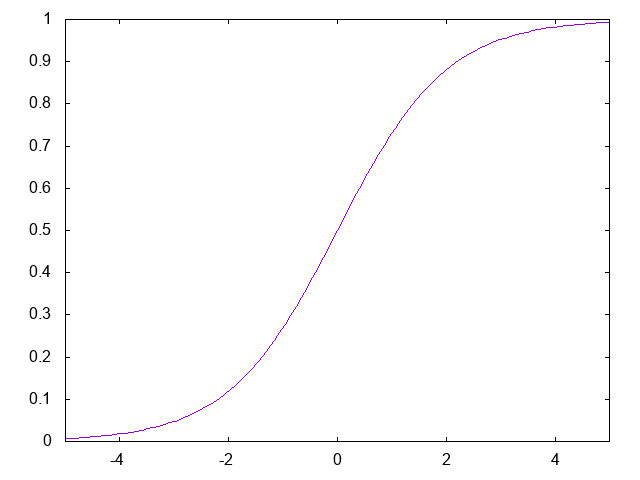
\includegraphics[scale=0.75]{bilder/logistic_reg_func}
\caption{Die logistische Funktion $p=\dfrac{1}{1+\exp(-x)}$ }
\end{figure}\\
Aufgrund der binären Art der Zielwerte ist es erstrebenswert dass die Ausgabewerte der Regressionsfunktion gegen 0 beziehungsweise 1 konvergieren. Optimal wäre also ein Funktionsverlauf von $f_\beta(\vec x_i)$ der dem Verlauf der Vorzeichenfunktion möglichst ähnlich ist (Siehe Abbildung 3.2), solange diese auf einen Wertebereich von $[0,1]$ transformiert wäre. Die $\sign(z(\vec x_i))$ selbst ist für die logistische Regression allerdings ungeeignet, da sie nicht stetig und damit nicht differenzierbar ist. Die Differenzierbarkeit ist jedoch eine Voraussetzung für die Optimierung der Funktion, was im nachfolgendem Abschnitt 3.2.2 näher erörtert wird.
Zusätzlich zu den anderen Vorteilen der logistischen Funktion ist ihre Ähnlichkeit zur Vorzeichenfunktion ein Grund sie für dichotome Entscheidungsprobleme zu verwenden.
\begin{figure}[ht]
\centering
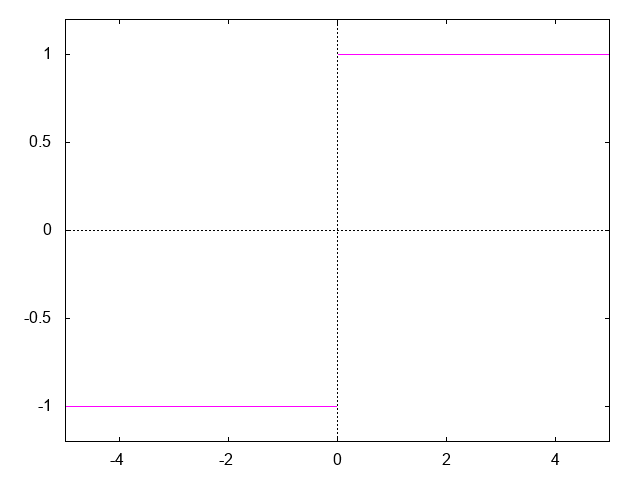
\includegraphics[scale=0.75]{bilder/sign}
\caption{Die Vorzeichenfunktion $q=\sign(x)$ }
\end{figure}\\
Wenn man jetzt also die Transformation der systematischen Komponente mit der logistischen Funktion durchführt erhält man die logistische Regressionsfunktion:
\begin{displaymath}
\pi(\vec x_i)= \dfrac{1}{1+\exp(z(\vec x_i))}
\end{displaymath}
Also genauer:
\begin{displaymath}
P(Y=1 | X=\vec x_i)=P(Y_i=1)=\frac{\exp(\beta_0+\vec x_i^T\beta)}{1+\exp(\beta_0+\vec x_i^T\beta)} = \frac{1}{1+\exp(-(\beta_0+\vec x_i^T\beta))}
\end{displaymath}
Die systemische Komponente $z(\vec x_i)=\beta_0 + \vec x_i^T\beta$ ist ein Prädiktor für $\pi(\vec x_i)$. Je größer $z(\vec x_i)$, desto größer auch $\pi(\vec x_i)$ und damit auch $P(Y=1|\vec x_i)$ \cite{BECK}.\newpage
\section{Lernen mit Logistischer Regression}
\subsection{Kostenfunktion und Maximum Likelihood}
Da das logistische Regressionsmodell dazu verwendet werden soll anhand gelernter Trainingsdaten Voraussagen für weitere, unbekannte Daten zu berechnen, ist es notwendig alle unbekannten Variablen entsprechend dem vorliegenden Datensatz anzupassen.
Um mit dem Modell möglichst korrekte Voraussagen treffen zu können müssen hierfür der Vektor der Koeffizienten $\beta$ und der Bias $\beta_0$ geschickt gewählt werden. Die Koeffizienten geben dabei die Bedeutsamkeit der einzelnen Ausprägungen der Variablen $X$ an, je größer $|\beta_i|, i \in 1..d$ desto größer sind auch die Auswirkungen der jeweiligen Ausprägung auf die Entscheidung \cite{FS}.
In der linearen Regression wird hierfür häufig die "`Methode der kleinsten Quadrate"' 
\begin{displaymath}
\sum_{i=1}^n(\pi(\vec x_i)-y_i)^2
\end{displaymath}
gewählt. Es werden die Werte für $\beta$ gewählt, welche möglichst kleine quadrierte Fehler machen. Somit ergibt sich die Minimierungsfunktion: 
\begin{displaymath}
\min_\beta \sum_{i_1}^n (\pi(\vec x_i)-y_i)^2
\end{displaymath}
Unter den üblichen Annahmen der linearen Regression ist die "`Summe der kleinsten Quadrate"' eine gute Schätzfunktion mit brauchbaren statistischen Eigenschaften \cite{WIL}.
Unter den Annahmen der logistischen Regression verliert diese Methode jedoch diese Eigenschaften. Die am häufigsten gewählte Methode die "`Summe der kleinsten Quadrate"' zu berechnen ist, unter Annahme dass die Fehlerterme normalverteilt sind, die Maximum Likelihood. Diese passt die unbekannten Variablen so an, dass die Chance, mit ihnen die gegebenen Daten darzustellen maximiert wird. Dies bildet auch die Grundlage zur Findung der unbekannten Variablen der logistischen Regression. Um diese Variablen bestimmen zu können bedarf es einer Funktion, der sogenannten Maximum Likeliehood Funktion. Sie drückt die Wahrscheinlichkeit aus in wie weit die gegebenen Daten die Variablen als Funktion darstellen. Die Maximum Likelihood Schätzer der Parameter sind dabei die Werte welche diese Funktion maximieren \cite{WIL}.
Aus der Maximum Likelihood Funktion ergeben sich zwei Kostenfunktionen, eine für den Fall $y_i =1$ und eine für den Fall $y_i=0$.
\begin{displaymath}
cost(\pi(\vec x_i), y_i)= \begin{cases}
-\log(\pi(\vec x_i)) & \text{wenn } y_i=1\\
-\log(1-\pi(\vec x_i)) & \text{wenn } y_i=0
\end{cases}
\end{displaymath}
Da $y_i$ immer entweder 0 oder 1 ist, kann man die Kostenfunktionen auch wie folgt zusammenfassen:
\begin{displaymath}
cost(\pi (\vec x_i), y_i) = y_i \cdot -\log(\pi(\vec x_i)) + (1-y_i) \cdot -\log(1-\pi(\vec x_i))
\end{displaymath}
Die Kostenfunktion über alle Eingaben lautet damit \cite{HER}:
\begin{displaymath}
J(\beta)=\dfrac{1}{n} \cdot \sum_{i=1}^n cost(\pi(\vec x_i), y_i) = \dfrac{1}{n} \cdot \sum_{i=1}^n y_i \cdot -\log(\pi(\vec x_i)) + (1-y_i) \cdot -\log(1-\pi(\vec x_i))
\end{displaymath}
\subsection{Gradientenabstiegsverfahren}
Das Gradientenabstiegsverfahren (Stochastic Gradient Descent, kurz SGD) ist ein Lernverfahren für Modelle mit nichtlinearen Parametern im Modellausgang. Es wird in statischen neuronalen Netzen dafür verwendet mittels eines Algorithmus' die Koeffizienten zu adaptieren. Ziel des Lernverfahrens ist es die Koeffizienten so anzupassen, dass die Abweichung  zwischen dem $y_i$ Wert der eingegebenen Variable und der Ausgabe $\pi(\vec x_i)$ möglichst gering ist. Diese Abweichung bezeichnet man als Ausgangsfehler \cite{IV}:
\begin{displaymath}
e_{\beta}(\vec x_i , y_i)=y_i-\pi(\vec x_i)
\end{displaymath}
Dieses Optimierungsproblem lässt sich wie folgt iterativ approximieren:
\begin{figure}[ht]
\centering
\begin{algorithmic}[1]
\STATE Wähle Startpunkt $\beta^{(0)}$
\STATE Iterationsindex $l \leftarrow 0$
\REPEAT
\STATE Bestimme Suchrichtung $s^{(l)}$
\STATE Bestimme skalare Schrittweite $\eta^{(l)} > 0$
\FOR {$i=0$ to $d$}
\STATE Bestimme $\beta_i^{(l+1)} = \beta_i^{(l)} + \eta^{(l)} \cdot s^{(l)}$
\ENDFOR
\STATE $l=l+1$
\UNTIL Abbruchbedingung erfüllt
\end{algorithmic}
\caption{Basisalgorithmus für SGD}
\end{figure}\\
Die einzelnen Abstiegsverfahren, wie zum Beispiel das Newton-, das Gradienten- oder das Konjugierte Gradientenverfahren unterscheiden sich in ihrer Struktur nur durch die Bestimmung der Suchrichtung $s^{(l)}$\cite{PAPA}. In Abbildung 3.4 ist der Verlauf des SGD für eine zweidimensionale Variable $\vec x_i$ zu sehen. Hier bei kann man erkennen dass sich die Länge der Schrittweiten der einzelnen Durchläufe des Algorithmus verkürzen, was auf eine dynamische Lernrate $\eta$ schließen lässt.\\\\
\begin{figure}[ht]
\centering
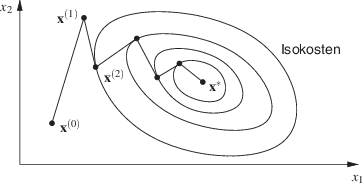
\includegraphics[scale=1.7]{bilder/SGD}
\caption{Beispielhafter Verlauf des Algorithmus im zweidimensionalen Fall}
\end{figure}\newpage
Voraussetzung für die Abstiegsrichtung ist es, dass für ein genügend kleines $0 < \eta^{(l)} < \tilde{\eta}^{(l)}$ die Gleichung 
\begin{displaymath}
f_{\beta}(\vec x + \eta^{(l)} \cdot s^{(l)}) < f_{\beta}(\vec x)
\end{displaymath} erfüllt ist.
Eine Hinreichende Bedingung dafür ist, dass die Suchrichtung und der Gradient $g_\beta^{(l)}(\vec x) = \bigtriangledown f_\beta^{(l)}(\vec x)$, also die Orthogonale auf dem Vektor $\vec x$, einen stumpfen Winkel zueinander bilden. Es gilt also als Hinreichende Bedingung \cite{PAPA}:
\begin{displaymath}
s^{(l)^T} \cdot g_\beta^{(l)}(\vec x) < 0
\end{displaymath}
In Abbildung 3.5 ist die Beziehung zwischen Gradienten, dem Vektor $\vec x$ und der Abstiegsrichtung noch einmal anschaulich dargestellt.\\
\begin{figure}[ht]
\centering
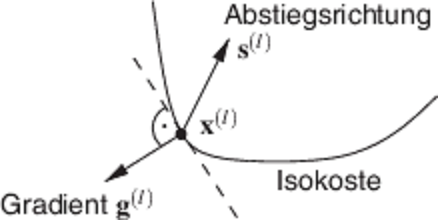
\includegraphics[scale=1]{bilder/gradient}
\caption{Beziehung zwischen Gradient und Abstiegsrichtung}
\end{figure}\\
Um nun die Funktion zu minimieren, formal $\min f_\beta(\vec x)$, kann das mehrdimensionale Problem durch eine Hilfsfunktion 
\begin{displaymath}
F(\varepsilon) = f(\vec x^* +e \cdot \sigma)
\end{displaymath}
in ein eindimensionales Problem umgewandelt werden. $\vec x^*$ bezeichnet hier ein lokales Minimum der Funktion $f_\beta(\vec x)$, $sigma$ ist ein beliebiger Vektor mit der gleichen Dimension wie $\vec x^*$ und $\varepsilon$ ist die für die Funktion eingeführte Variable. Nun hat die Funktion $f_\beta$ an der Stelle $\vec x^*$ genau dann ein lokales Minimum, wenn $F(\varepsilon)$ für jeden beliebigen Vektor $\sigma \in \mathbb{R}^d$ an der Stelle $\varepsilon^*=0$ auch ein lokales Minimum aufweist. Dazu muss gelten:
\begin{displaymath}
F'(0)=\sigma^T \cdot \bigtriangledown f_\beta(\vec x^*) = 0
\end{displaymath}
was genau dann erfüllt ist, wenn:
\begin{displaymath}
\bigtriangledown f_\beta(\vec x^*)=0
\end{displaymath}
Diese Notwendige Bedingung erster Ordnung ist für alle stationären Punkte, also von allen lokalen Minima, Maxima und Sattelpunkten erfüllt und erlaubt die Definition einer Abbruchbedingung durch das Vorgeben eine Toleranzgrenze $\mu > 0$. Abgebrochen wird der Algorithmus wenn 
\begin{displaymath}
\parallel g_\beta^{(l)} \parallel < \mu
\end{displaymath}
Bei dem SGD Verfahren wird als Suchrichtung $s^{(l)}$ der negative Gradient $-g_\beta^{(l)}(\vec x)$ verwendet. Dadurch erfüllt sich  automatisch die Hinreichende Bedingung für alle nichtstationären Punkte sicher, denn \cite{PAPA}: 
\begin{displaymath}
s^{(l)^T} \cdot g_\beta^{(l)} = - \parallel g_\beta^{(l)} \parallel^2 < 0
\end{displaymath}
\subsection{Zusammenführen der Funktionen}
Das Ziel der logistischen Regression mit SGD ist es, die Kostenfunktion $J(\beta)$ zu minimieren. Aus den Erkenntnissen in Abschnitt 3.2.2 lässt sich entnehmen, dass für die Anpassung der Koeffizienten $\beta^{(l+1)}$ der negative Gradient verwendet wird. Dieser berechnet sich nach 3.2.1 durch die Partielle Ableitung der Kostenfunktion nach $\beta_i$ für alle $\vec x_i, i \in [1,n]$:
\begin{displaymath}
\dfrac{\partial}{\partial \beta_i} J(\beta) = - \frac{1}{n} \sum_{i=1}^n (\pi(\vec x_i) - y_i)\cdot \vec x_i
\end{displaymath}
beziehungsweise für den direkten Fall $\beta_i$ mit $\vec{x_i}$:
\begin{displaymath}
\dfrac{\partial}{\partial \beta_i} cost(\pi(\vec x_i),y_i) = (y_i -\pi(\vec x_i))\cdot \vec x_i
\end{displaymath}
Somit werden die Koeffizienten nach mit allen Variablen $\vec x_i, i \in [1,n]$ durch folgenden Term angepasst \cite{HER}:
\begin{displaymath}
\beta^{(l+1)} = \beta^{(l)} + \eta^{(l)} \cdot \frac{1}{n} \sum_{i=1}^n (y_i-\pi(\vec x_i)) \cdot \vec x_i
\end{displaymath}
Hierbei kann $n$ auch durch eine beliebige Variable $m\text{ . }0< m < n$ ersetzt werden, wodurch eine Batch Anpassung, also eine Anpassung der Koeffizienten nach $m$ Schritten durch das Mittel der Kostenfunktionen entsteht:
\begin{displaymath}
\beta^{(l+1)} = \beta^{(l)} + \eta^{(l)} \cdot \frac{1}{m} \sum_{i=l\cdot m + 1}^{(l+1) \cdot m} (y_i-\pi(\vec x_i)) \cdot \vec x_i
\end{displaymath}
Für den Durchlauf mit einem Update nach jeder Variable $\vec x_i$ (Batchsize $=1$) gilt \cite{COH}:
\begin{displaymath}
\beta^{(l+1)} = \beta^{(l)} + \eta^{(l)} \cdot (y_i-\pi(\vec x_i)) \cdot \vec x_i
\end{displaymath}
Die Anpassung der Koeffizienten kann durch die Erweiterung der Kostenfunktion noch weiter verbessert werden, um beispielsweise einer Überanpassung der Koeffizienten entgegenzuwirken: \begin{displaymath}
\min_\beta \left( \frac{1}{n} \sum_{i=1}^n (y_i - \pi(\vec x_i))\cdot \vec x_i +C \cdot R(\beta)\right) 
\end{displaymath}
Wobei $C \in \mathbb R$ ein Hyperparameter zur Gewichtung ist, der fest gewählt werden muss. Dies geschieht zumeist durch das Testen verschiedener Werte, sodass hier ein Ansatz zur Parallelisierung entsteht. $R(\beta)$ beschreibt einen Regularisierungsterm, auf den im Kapitel 3.3 näher eingegangen wird.
\section{Regularisierungsmethoden}
Regularisierung ist jede Modifikation die an einem Lernalgorithmus vorgenommen wird um den Generalisierungsfehler, jedoch nicht seinen Trainingsfehler zu reduzieren \cite{GOO}.\\
Wenn ein Lernalgorithmus mit logistischer Regression mit einem Datensatz trainiert wird, kann dieser auf den gegebenen Daten ausreichend gute Voraussagen treffen \cite{NG}. Es kann jedoch passieren, dass die Häufigkeit von richtigen Voraussagen auf neuen, von dem Algorithmus nicht gelernten Daten drastisch sinken. Man bezeichnet das Modell dann als "`overfitted"' (überangepasst). Das bedeutet, dass der Algorithmus zwar die vorgegebenen Trainingsdaten für Voraussagen gelernt hat, aber von dem gelernten Modell nicht generalisieren kann. Ein Beispiel dafür ist in Abbildung 3.6 und 3.7 zu sehen.
\begin{figure}[ht]
\centering
	\begin{minipage}[b]{.4\linewidth}
  		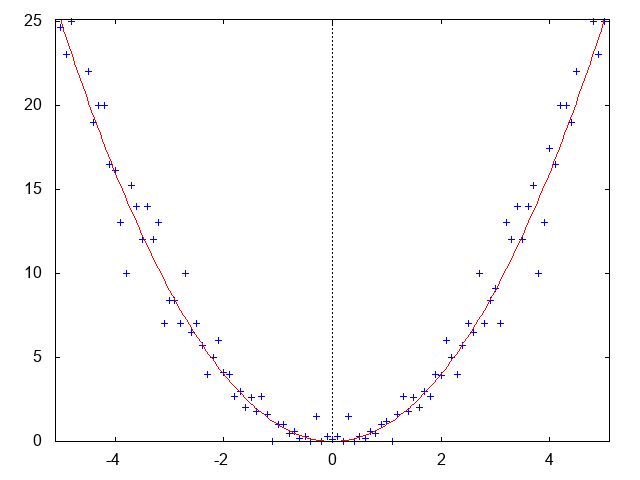
\includegraphics[scale=0.4]{bilder/normal}
  		\caption{Normale Regressionsgrade}
  	\end{minipage}
  	\hspace{.1\linewidth}% Abstand zwischen Bilder
  	\begin{minipage}[b]{.4\linewidth}
  		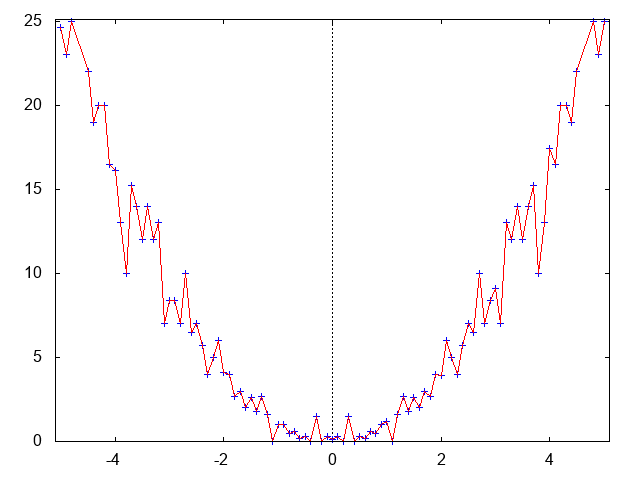
\includegraphics[scale=0.4]{bilder/overfitting}
		\caption{Overfitting des Modells}
	\end{minipage}
	
\end{figure}\\
Um besagtes Overfitting zu vermeiden können zum einen möglichst repräsentative Trainingsdatensätze gewählt werden, zum anderen kann die Minimierungsfunktion mit einem Regularisierungsterm erweitert werden.
Die Regularisierung soll zu hoch gewichtete Koeffizienten bestrafen oder nicht die Gewichtung für unwichtige Koeffizienten reduzieren.
Hierfür werden nachfolgend zwei Methoden vorgestellt.
\subsection{LASSO}
L1-Regularisierung (Least Absolute Shrinkage and Selection Operator, kurz \textbf{LASSO}) ist die l1 Norm der Koeffizienten, definiert als lineare Funktion durch:
\begin{displaymath}
R(\beta) = \parallel \beta \parallel_1 = \sum_{i}^n|\beta_i|
\end{displaymath}
Man nennt die l1 Norm auch die Manhattan Distanz, also die Distanz die benötigt wird um von einem Punkt zu einem anderen zu gelangen, nur mit Laufrichtungen parallel zu einer der Achsen des Koordinatensystems. L1-Regularisierung ist schwierig zu optimieren, da die Betragsfunktion an der Stelle 0 nicht differenzierbar ist. Eine Regularisierung mit LASSO führt zu einem spärlichen Koeffizientenvektor mit einigen großen und vielen kleinen Gewichten ($=0$), so das wenige Features gewählt werden. Die Verteilung der Gewichte entspricht somit einer Laplace-Verteilung \cite{JUR}. In Abbildung 3.x wird eine Regularisierung mit L1 dargestellt.
\subsection{Ridge Regression}

L2-Regularisierung (Ridge Regression) ist die quadrierte l2 Norm der Koeffizienten, definiert durch:
\begin{displaymath}
R(\beta)= \parallel \beta \parallel_2^2= \dfrac{1}{2} \sum_{i}^n \beta_i^2
\end{displaymath}
Die Konstante $\frac{1}{2}$ dient hier der einfacheren Berechnung der Ableitung für die Optimierung und wird über die Anpassung von $C$ kompensiert. L2 entspricht der Euklidischen Distanz des Koeffizientenvektors zum Ursprung. Regularisierung mit Ridge Regression führt zu deutlich kleineren Koeffizienten und damit zu weniger überangepassten einzelnen Features. Die Verteilung des Koeffizientenvektors entspricht einer Gauß'schen Verteilung mit Median $\mu = 0$ und Varianz $ 2 \sigma^2 = 1$ \cite{JUR}.
Sei 
\begin{displaymath}
\dfrac{1}{\sqrt{2\pi \sigma_j^2}}\exp\left(-\dfrac{(\beta_j-\mu_j)^2}{2\sigma_j^2}\right)
\end{displaymath}
die Gauß-Verteilung des Koeffizienten $\beta_j$. Wenn man nun jeden Koeffizienten mit der Gauß'schen Verteilung der Koeffizienten multipliziert, erhält man folgenden Term:
\begin{displaymath}
\tilde{\beta} = \max_{\beta} \prod_{i=1}^n P(y_i | \vec x_i) \cdot \prod_{j=1}^d \dfrac{1}{\sqrt{2\pi \sigma^2}}\exp\left(-\dfrac{(\beta_j-\mu_j)^2}{2\sigma_j^2}\right)
\end{displaymath}
Im logarithmischen Raum, mit $\mu =0$ und $2\sigma^2 = 1$ verhält dieser sich gleich dem Term: 
\begin{displaymath}
\tilde{\beta} = max_\beta \sum_{i=1}^n logP(y_1 | \vec x_i)-C \cdot \sum_{j=1}^d \beta_j^2
\end{displaymath}
Welcher äquivalent zu unserer Minimierungsfunktion aus 3.2.3 ist \cite{JUR}.
\subsection{Zusammenfassung der Regularisierungsmethoden}
